\documentclass{article}

\usepackage[margin=3cm]{geometry}

\usepackage{tikz-bagua}
\usetikzlibrary{math}

\input{binhex}

\usepackage{makeidx} 

\makeindex  

\title{TikZ-Bagua Package}
\author{WANG Xu \\ cwangx@hotmail.com}
\date{\today~v1.01}

\begin{document}

\maketitle

\section{Introduction}

The \verb+TikZ-Bagua+ package mainly using \verb+TikZ+, by \verb+xparse+, \verb+xstring+, \verb+bitset+ and \verb+xintexpr+, defines the Grand Terminus \cite{Legge} \verb+\taiji+ and \verb+\xtaiji+ for newer method, \verb+\liangyi+ for the Two Elementary Forms, \verb+\sixiang+ for the Four Emblematic Symbols, \verb+\bagua+ for the Eight Trigrams and \verb+\Bagua+ for Sixty-four Hexagrams,  in \emph{The I Ching}, without require special fonts.

\section{Usage methods}

The last argument of all defined macros is optional \verb|scale|, and default $1$.

\subsection{The Grand Terminus (the \emph{Taiji})}

Thanks to netizens, the default is same as in ancient books without \emph{the Fish Eyes}, show its by macro with star.
For reason that there are some formed by semi-circles, so add \verb+\xtaiji+ for it, with (or without) star.

\verb+\taiji [<scale>]+\index{taiji@\verb+\taiji+}, \verb+\taiji* [<scale>]+\index{xtaiji@\verb+\xtaiji+}.

\verb+\xtaiji [<scale>]+\index{taiji@\verb+\taiji+}, \verb+\xtaiji* [<scale>]+\index{xtaiji@\verb+\xtaiji+}.

The four above macros show \taiji \taiji* \xtaiji \xtaiji*.

\subsection{The Two Elementary Forms (the \emph{Liangyi})}
\verb+\liangyi {<bin>} [<scale>]+\index{liangyi@\verb+\liangyi+}.

We can obtain \liangyi{1} and \liangyi{0} by \verb+\liangyi{<bin>}+ getting $1$ and $0$, respectively.


\subsection{The Four Emblematic Symbols (the \emph{Sixiang})}
\verb+\sixiang {<bin>} [<scale>]+\index{sixiang@\verb+\sixiang+}, \verb+\sixiang* {<dec>} [<scale>]+\index{sixiang*@\verb+\sixiang*+}.

The Four Emblematic Symbols obtained from \verb+\sixiang{<bin>}+ by getting the binary number of $3,2,1,0$, and \verb+\sixiang*{<dec>}+ for decimal.

\begin{center}
	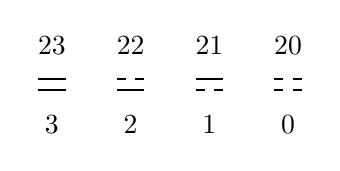
\begin{tikzpicture}
		\foreach \j in {3,2,1,0}
		{
			\node at (3-\j,-0.5) {$\j$};
			\node at (3-\j,0.5) {\nbinary{2}{\j}};
			\node at (3-\j,0) {\sixiang*{\j}};
		}
	\end{tikzpicture}
\end{center}

\subsection{The Eight Trigrams (the \emph{Bagua} with three lines)}
\verb+\bagua {<bin>} [<scale>]+\index{bagua@\verb+\bagua+}, \verb+\bagua* {<dec>} [<scale>]+\index{bagua*@\verb+\bagua*+}.

The Eight Trigrams obtained from \verb+\bagua{<bin>}+ by getting the binary number of $7,6,\dots,0$, and \verb+\bagua*{<dec>}+ for decimal.

\begin{center}
	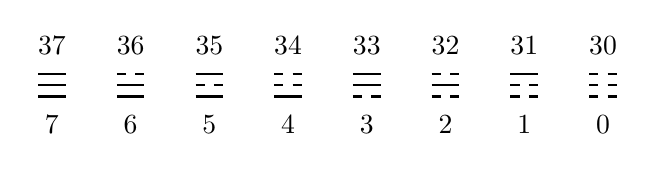
\begin{tikzpicture}
		\foreach \j in {7,6,...,0}
		{
			\node at (7-\j,-0.5) {$\j$};
			\node at (7-\j,0.5) {\nbinary{3}{\j}};
			\node at (7-\j,0) {\bagua*{\j}};
		}
	\end{tikzpicture}
\end{center}

\subsection{The Sixty-four Hexagrams (the \emph{Bagua} with six lines)}
\verb+\Bagua [<2,8>]{<bin,oct>} [<scale>]+\index{Bagua@\verb+\Bagua+}, \verb+\Bagua* {<dec>} [<scale>]+\index{Bagua*@\verb+\Bagua*+}.

The Sixty-four Hexagrams obtained from \verb+\Bagua{<bin>}+ by getting the binary number of $63,62,\dots,0$, \verb+\Bagua[8]{<oct>}+ for octal number $77,76,\dots,0$, and \verb+\bagua*{<dec>}+ for decimal.

We list all the Sixty-four Hexagrams here, in which the above number is binary, the below is decimal and octal.

\begin{center}
	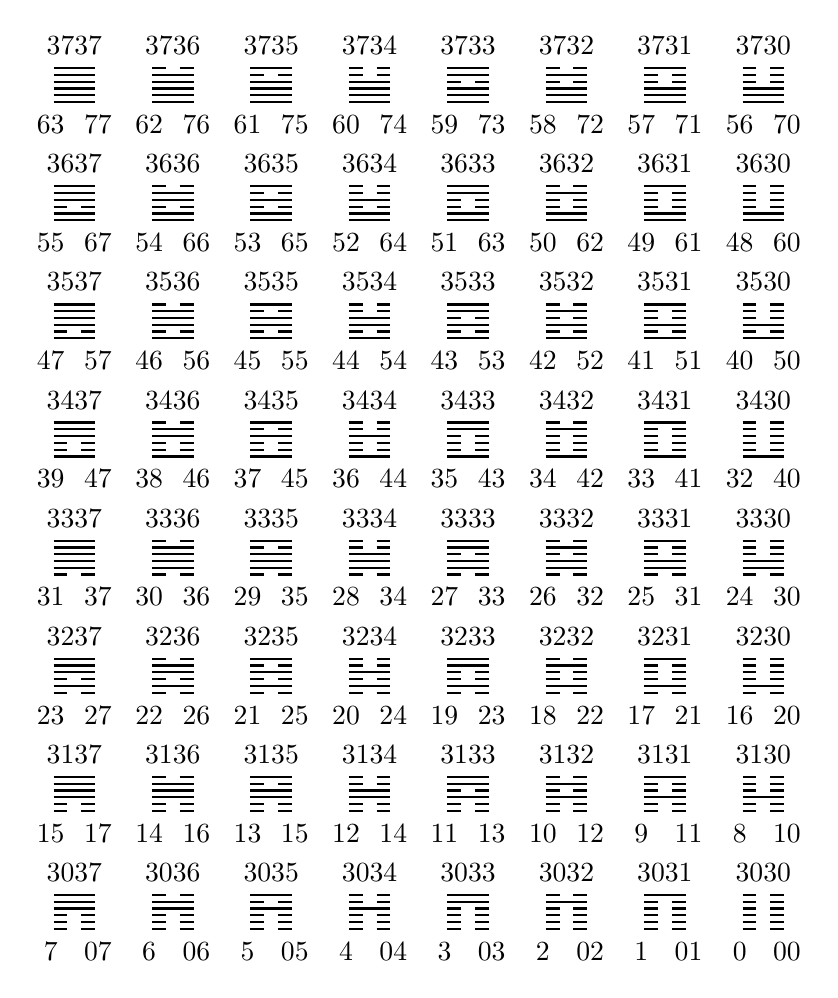
\begin{tikzpicture}
		\foreach \j in {7,6,...,0}
		{
			\foreach \k in {7,6,...,0}
			{
				\node at (7*1.25-1.25*\k-0.3,1.5*\j-0.5) {\pgfmathparse{int(8*\j+\k)}\pgfmathresult};
				\node at (7*1.25-1.25*\k+0.3,1.5*\j-0.5) {\j\k};
				\node at (7*1.25-1.25*\k,1.5*\j+0.5) {\nbinary{3}{\j}\nbinary{3}{\k}};
				\node at (7*1.25-1.25*\k,1.5*\j) {\Bagua[8]{\j\k}[1.5]};
			}
%			\node at (7-\j,0) {$\j$};
%			\node at (7-\j,-0.5) {\nbinary{3}{\j}};
%			\node at (7-\j,-1) {\bagua*{\j}};
		}
	\end{tikzpicture}
\end{center}

\section{Versions}
\subsection*{v1.01~2022.08.04}
Revise \verb+\taiji+ to show the Grand Terminus in ancient books, add \verb+\xtaiji+ for later, fix some bugs.

\subsection*{v1.0~2021.10.17}
Release \verb+TikZ-Bugua+ v1.0.

\begin{thebibliography}{9}
    \bibitem {Legge} James Legge (Trans.). The I Ching, Second Edition. Dover Publications, Inc.
\end{thebibliography}

\printindex

\end{document}